\begin{center}
\Huge
Mere om andengradspolynomier
\end{center}
\section*{Grafer for andengradspolynomier}
\stepcounter{section}


For en god ordens skyld giver vi en definition på et andengradspolynomium.
\begin{defn}[Andengradspolynomium]
	En funktion $f$ på formen
	\begin{align*}
		f(x) = ax^2+bx+c,
	\end{align*}
	hvor $a \neq 0$ kaldes for et andengradspolynomium.
\end{defn}
Vi skal kunne bruge koefficienterne i et andengradspolynomium til at afgøre, hvordan grafen for polynomiet ser ud. For koefficienterne gælder der:
\begin{itemize}
	\item[$\cdot$] Tallet $c$ er skæringen med $y$-aksen.
	\item[$\cdot$] Tallet $b$ fortæller os, om parablen er voksende eller aftagende i skæringen
	med $y$-aksen. Hvis $b > 0$, så er parablen voksende, og hvis $b<0$, så er parablen 
	aftagende.
	\item[$\cdot$] Tallet $a$ fortæller os, om parablens arme vender op eller ned. Hvis 
	$a > 0$, så vender armene op ad, og hvis $a < 0$, så vender armene nedad. 
\end{itemize}
På Figur \ref{fig:andenpolys2} kan vi se to parabler. 
\begin{figure}[H]
	\centering
	\resizebox{0.45\textwidth}{!}
	{
	\begin{tikzpicture}
		\begin{axis}[
		axis lines = middle,
		xlabel = $x$, ylabel = $y$,
		xmin = -2, xmax = 6, ymin = -5, ymax = 4,
		ytick = {-2}, xtick = {0},
 		]
			\addplot[thick, samples = 1000, color = olive] {x^2-3*x-2};
			\node[anchor = west] at (axis cs: 4,-2) {$a > 0$};
			\node[anchor = west] at (axis cs: 4,-2.8) {$b < 0$};
			\node[anchor = west] at (axis cs: 4,-3.6) {$c = -2$};
		\end{axis}
	\end{tikzpicture}
	}
	\resizebox{0.45\textwidth}{!}
	{
	\begin{tikzpicture}
		\begin{axis}[
		axis lines = middle,
		xlabel = $x$, ylabel = $y$,
		xmin = -2, xmax = 3, ymin = -2, ymax = 4,
		ytick = {1}, xtick = {0},
 		]
			\addplot[thick, samples = 1000, color = olive] {-x^2+2*x+1};
			\node[anchor = west] at (axis cs: 1,3.8) {$a < 0$};
			\node[anchor = west] at (axis cs: 1,3.3) {$b > 0$};
			\node[anchor = west] at (axis cs: 1,2.8) {$c = 1$};
		\end{axis}
	\end{tikzpicture}
	}
	\caption{To parabler}
	\label{fig:andenpolys2}
\end{figure}

\section*{Skæringer mellem parabler}
\stepcounter{section}

Ønsker vi at bestemme skæringspunkterne mellem to parabler, så gøres dette tilsvarende med at finde skæringer mellem linjer. Udtrykkende for parablernes andengradspolynomier sættes lig hinanden og ligningen løses. Vi skal dog her være opmærksomme på, at vi i de fleste tilfælde nemmest løser denne ligning ved at bruge diskriminantformlen.

\begin{exa}
To polynomier $f$ og $g$ er givet ved
\begin{align*}
	f(x) = 2x^2 + 3x - 3
\end{align*}
og
\begin{align*}
	g(x) = x^2 + x + 5
\end{align*}
og vi ønsker at bestemme skæringspunkterne mellem deres grafer. Vi sætter derfor udtrykkene lig hinanden og isolerer alt på venstresiden.
\begin{align*}
	f(x) = g(x)\ &\Leftrightarrow \ 2x^2 + 3x - 3 = x^2 + x + 5 \\
	&\Leftrightarrow \ x^2 + 3x - 3 = x + 5 \\
	&\Leftrightarrow \ x^2 + 2x - 3 = 5 \\
	&\Leftrightarrow \ x^2 + 2x - 8 = 0.
\end{align*}
Vi kan nu anvende diskriminantformlen til at løse ligningen
\begin{align*}
	d = 2^2 - 4\cdot 1 \cdot (-8) = 4 +32 = 36.
\end{align*}
Vi får altså løsningerne
\begin{align*}
	x_1 = \frac{-2 + \sqrt{36}}{2\cdot 1} = \frac{-2+6}{2} = 2
\end{align*}
og 
\begin{align*}
	x_2 = \frac{-2-6}{2} = - 4.
\end{align*}
Disse tal sættes nu ind i enten $f$ eller $g$. Vi bruger $g$:
\begin{align*}
	g(2) = 2^2 + 2 + 5 = 11
\end{align*}
og 
\begin{align*}
	g(-4) = (-4)^2 -4 + 5 = 16 -4 + 5 = 17
\end{align*}
Skæringspunkterne er derfor $(2,11)$ og $(-4,17)$.
\end{exa}

\subsection*{Opgave 1}

Parablen for et andengradspolynomium $p$ er givet.
\begin{enumerate}[label=\roman*)]
	\item Aflæs rødderne for $p$.
	\item Bestem tallene $p(3)$ og $p(-4)$.
	\item Løs ligningerne $p(x) = 5$ og $p(x) = -6$. Er $p$ injektiv?
	\item Bestem $c$-værdien for $p$.
	\item Bestem fortegnet for både $a$ og $b$-værdien for $p$.
\end{enumerate}

\begin{center}
	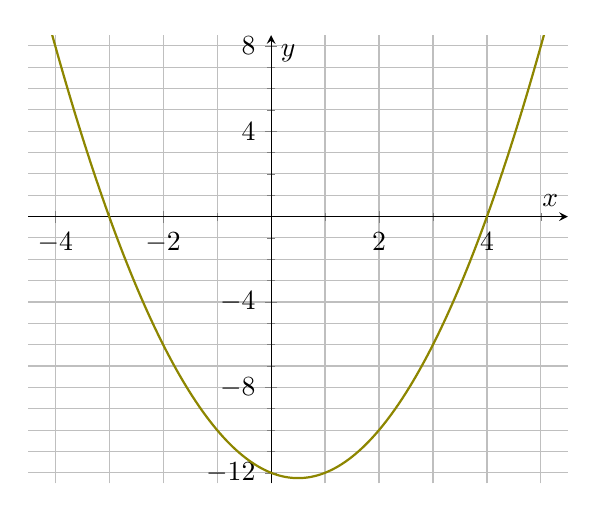
\begin{tikzpicture}
	\begin{axis}[
	axis lines = center,
	xmin = -4.5, xmax = 5.5,
	ymin = -12.5, ymax = 8.5,
	grid = both, 
	xlabel = $x$, ylabel = $y$, 
	xtick = {-4,-2,...,4,6},
	ytick = {-12,-8,...,8,12},
	minor x tick num = 1,
	minor y tick num = 3,
	]
		\addplot[color = olive, thick, domain = -5:6, samples = 200] {(x+3)*(x-4)};
	\end{axis}
	\end{tikzpicture}
\end{center}

\subsection*{Opgave 2}
Et andengradspolynomium er givet ved
\begin{align*}
	p(x) = -2x^2 - 4x + 6 
\end{align*}
\begin{enumerate}[label=\roman*]
	\item Bestem $p(2)$ og $p(-1)$.
	\item Løs ligningen $p(x) = 0$. 
\end{enumerate}

\subsection*{Opgave 3}
\begin{enumerate}[label=\roman*)]
	\item Et andengradspolynomium $p(x) = x^2 + 4x + c$ går gennem punktet $P(2,15)$. Bestem tallet $c$.
	\item Et andengradspolynomium $p(x) = -3x^2 + bx + 3$ går gennem punktet $P(-1,4)$. Bestem tallet $b$.
\end{enumerate}

\subsection*{Opgave 4}
\begin{enumerate}
	\item Bestem skæringspunkterne mellem 
	$$f(x) = 3x^2 + 5x + 5$$ 
	og
	$$g(x) = 2x^2 -4x -15.$$
	\item Bestem skæringspunkterne mellem
	 $$f(x) = -x^2 + 6x -9$$
	 og 
	 $$g(x) = -2x^2 + 3x + 9.$$
\end{enumerate}

\subsection*{Opgave 5}
Et andengradspolynomium $p$ er givet ved
\begin{align*}
	p(x) = x^2 + bx +c 
\end{align*}
og opfylder, at $p(0) = 5$ og $p(2) = 5$.
\begin{enumerate}[label=\roman*)]
	\item Bestem tallene $b$ og $c$. 
\end{enumerate}
